%
% File acl2015.tex
%
% Contact: car@ir.hit.edu.cn, gdzhou@suda.edu.cn
%%
%% Based on the style files for ACL-2014, which were, in turn,
%% Based on the style files for ACL-2013, which were, in turn,
%% Based on the style files for ACL-2012, which were, in turn,
%% based on the style files for ACL-2011, which were, in turn, 
%% based on the style files for ACL-2010, which were, in turn, 
%% based on the style files for ACL-IJCNLP-2009, which were, in turn,
%% based on the style files for EACL-2009 and IJCNLP-2008...

%% Based on the style files for EACL 2006 by 
%%e.agirre@ehu.es or Sergi.Balari@uab.es
%% and that of ACL 08 by Joakim Nivre and Noah Smith

\documentclass[11pt]{article}
\usepackage{acl2015}
\usepackage{times}
\usepackage{url}
\usepackage{latexsym}
\usepackage{caption}
%
\usepackage{lipsum}                    
\usepackage{xargs}                     
\usepackage{graphicx}
\graphicspath{ {images/} }

\usepackage[pdftex,dvipsnames]{xcolor} 
\usepackage[colorinlistoftodos,prependcaption,textsize=tiny]{todonotes}
\newcommandx{\unsure}[2][1=]{\todo[linecolor=red,backgroundcolor=red!25,bordercolor=red,#1]{#2}}
\newcommandx{\change}[2][1=]{\todo[linecolor=blue,backgroundcolor=blue!25,bordercolor=blue,#1]{#2}}
\newcommandx{\info}[2][1=]{\todo[linecolor=OliveGreen,backgroundcolor=OliveGreen!25,bordercolor=OliveGreen,#1]{#2}}
\newcommandx{\improvement}[2][1=]{\todo[linecolor=Plum,backgroundcolor=Plum!25,bordercolor=Plum,#1]{#2}}
\newcommandx{\thiswillnotshow}[2][1=]{\todo[disable,#1]{#2}}

\newcommand{\tabref}[1]{\textit{Table \ref{#1}}}
\newcommand{\figref}[1]{\textit{Figure \ref{#1}}}
%
%\setlength\titlebox{5cm}

% You can expand the titlebox if you need extra space
% to show all the authors. Please do not make the titlebox
% smaller than 5cm (the original size); we will check this
% in the camera-ready version and ask you to change it back.

\title{Analysis of Tweet Generation as an Extractive Summarization Problem}

\author{First Author \\
  Affiliation / Address line 1 \\
  Affiliation / Address line 2 \\
  Affiliation / Address line 3 \\
  {\tt email@domain} \\\And
  Second Author \\
  Affiliation / Address line 1 \\
  Affiliation / Address line 2 \\
  Affiliation / Address line 3 \\
  {\tt email@domain} \\}

\date{}

\begin{document}
\maketitle
\begin{abstract}
\todo{Write abstract}
\end{abstract}


\section{Introduction}

Summarization of documents has been studied frequently, and the methods of doing so can be broadly classified as extractive and abstractive \cite{hahn2000challenges}. Extractive summarization identifies keywords and phrases from the original text and strings them together to form a summary, while abstractive summarization describes the content of the document in more general terms. Both summarization techniques work by identifying the most significant words in the document and using them for further processing. 

With the rise of the popularity of social media, message broadcasting sites have become the new means of communication, voicing opinions, broadcasting news, promotions and so on. Everyone including newspapers, channels, movies, government officials, entertainers, have established themselves on social media and regularly use it for news broadcasting and promotions. Twitter is such a public message broadcasting service with the constraint on the message being under 140 charachters. Since all posts on the website are public and a limited length, it has been termed as microblogging - messages, called tweets, that convey precise information about a given topic in a limited number of characters. \change{Terrible sentence}The nature of this website has made it popular for global discussions on current goings-on in the world, with an estimated 200 million tweets being tweeted per day.

The tweets are often used as a link to a new web page, that has more detailed information about the topic being discussed. This set up suggests that the web page, which might contain videos, images, or articles, blogs, and so on is being promoted with the use of the tweet. In the case of articles, intuitively, the tweet seems to be an indicative, informative, or critical summary of the article being promoted. 

We used data from tweets and the connecting articles and explore the possibility of generating tweets using an extractive summarization algorithm. However, after running analyses on the data we discovered that it does not make sense to model tweet generation from articles as an extractive summarization problem. The size of the tweet is too small to be able to form a coherent sentence for the tweet. \improvement{Add classification by intent and use of formality lexicons}

\section{Background and Related Work}
\change{Add papers:

* summarization evaluation papers

* papers on classifying tweets based on intent?

* Add some glue at beginning of section}

There has been work on using user ratings prediction for stylistic surface realisation \newcite{dethlefs2014cluster}. The study used ratings by users for generated texts along three axes of style, colloquialism, naturalness and politeness. The study then clustered users according to their ratings, and used stylistic predictions from this cluster towards the surface realization of new text. The three axes chosen were fairly arbitrarily, and may not have been completely independent. However, the concept of rating documents according to the stylistic characteristics of the text and using this stylistic information to rate the newly generated text is something that can be explored further. 

\newcite{brooke2012building} describe the process of building a formality lexicon by analyzing the stylistics of text. They calculate formality scores for words and sentences by training a model on a large corpus based on the appearance of words in specific documents. Their model represents words as vectors and the formal and informal seeds appear in opposite halves of the graphs, suggesting that we can use these seeds to determine if an article is formal or informal. \newcite{brooke2013multi} used an LDA based model using a similar idea of seed words for getting stylistic rankings for documents. The documents were ranked for styles such as literary, colloquial, subjective, concrete, and so on. 

There have also been studies specific to Twitter data, for classifying and summarizing text, intents, etc. \newcite{ghosh2011entropy} classified the retweeting activity of users based on entropy. The study considered the occurrence of the same URL in a different tweet as a ‘retweet’, and was able to separate the tweets as automatic or robotic retweeting, campaigns, news, blogs and so on. The study shows some interesting trends of retweeting activity for each of these cases. In another study,\newcite{chen2012extracting}, were able to extract sentiment expressions based on their corpus of tweets, that resulted in extraction of both formal and slang sentiment bearing words.

\unsure{More details on each paper?}
Mirco-blogging sites, easy access to Internet and the popularity of social media offers an opportunity to analyze data that comprises of statements from a huge number of users. Twitter is such a platform and has gained millions of users by now, and is hugely popular platform now for announcements, voicing opinions, promotions and so on. This data has been used for event summarization studies. \newcite{o2010tweetmotif} uses topic summarizations for a given search for better browsing. \newcite{chakrabarti2011event} generate an event summary by learning the event using a Hidden Markov Model over the tweets describing it. \newcite{wang2014socially} generate a coherent event summary by treating summarization as an optimization problem for topic cohesion. \newcite{inouye2011comparing} compare multiple summarization techniques to generate a summary of multi-post blogs on Twitter.

There has also been an attempt at generating tweets, texts of 140 characters using different text summarization techniques by  \newcite{lloret2013towards}. Summarization systems were used to summarize texts to sentences and then were compared against each other, evaluated using the ROUGE metric for evaluation. The ROUGE-1, ROUGE-2 and ROUGE-L metrics were used and the tweets were compared against an ideal summary. ROUGE is better when used with multiple reference texts and is not meant to be used at the sentence level. Thus the evaluation is done using the unigram, bigram and longest common subsequence matching techniques used in ROUGE-1, 2 and L. None of these techniques evaluate the fluency of the text, which is generally not expected from extractive summarization. 

To the best of our knowledge, only \newcite{lofi2012iparticipate} aim at generating tweets based on data from documents related to the topic. The system proposed uses keyword extraction techniques to generate tweets containing links to the article, hashtags based on the topic from documents and summarized content of the document. The study does not give details of implementation or evaluation of the system. Moreover, after the hashtags and the url, the Twitter constraint of 140 characters leaves room for few words in the generated tweet.


\section{Data Extraction and Preprocessing}

\subsection{Using Twitter for Data Extraction}

As mentioned earlier, there have been numerous studies that used data from the public Twitter feeds. However, since none of the datasets used in these studies contained tweets and related articles promoted by these tweets separated into categories as required for this study, we extracted data directly from the site.

\subsection{Extracting Data}

Data was extracted from Twitter using the Twitter REST API using 51 search terms, or ‘hashtags’. These hashtags were chosen from a range of topics including pop culture,  international summit meetings discussing political issues, lawsuits and trials, social issues and health care issues. All these hashtags were ‘trending’ (being tweeted about at a high rate) at the time of extraction of the data. To give the data some variety, the data was extracted over the course of 15 days in November, which gave us multiple news stories to choose from for the search terms. A few examples of the search terms are shown in \tabref{tab:searchterms} Only English tweets were extracted since the study is limited to English. In the beginning, about 30,000 tweets were extracted, and more than half of these tweets, around 16,000 contained URLs referencing some news articles, photos on photo sharing sites, and videos. The hashtags were chosen to maximise the number of articles related to the tweets. Hence, a lot of topics that were chosen were being tweeted about by news agencies and other popular news sources. \improvement{Can be compressed if required}

% \begin{table}[h]
% \begin{tabular}{lll}
% \hline
% \#winteriscoming         & \#rosetta              & \#moneyball                          \\ 
% \#apec2014               & \#oscarpistorius       & \#bahamas               \\
% \#G20                    & \#johnoliver           & \#philae               \\
% \#annefrank              & \#putin                & \#lestweforget         \\
% \#cdnpoli                & \#android              & \#syria                \\
% \#mangalayan             & \#montythepenguin      & \#beenrapedneverreported             \\
% \#playingitmyway         & \#MarysvilleShooting   & \#1989                 \\
% \#GOP                    & \#ottawashootings      & \#canadachinatradedeal \\
% \#ausvssa                & \#BBCSyriaWars         & \#mentalhealth         \\
% \#lollipopupdate         & \#berlinwall           & \#memorialday          \\
% \#nexus6                 & \#RobertONeill         & \#nycmarathon          \\
% \#ebola                  & \#TaylorSwift          & \#pointergate          \\
% \#obamacare              & \#apec                 & \#theforceawakens      \\
% \#1wtc                   & \#netneutrality        & \#erdogan              \\
% \#snowstorm              & \#instellar            & \#buffaloSnow          \\
% \#lollipop               & \#cometlanding         & \#KevinVickers         \\
% \#haiyan                 & \#ferguson             & \#abercrombieandfitch  \\
% \#harrypotter            & \#betterstarwarstitles & \#ghomeshi             \\ \hline
% \end{tabular}
% \end{table}

\begin{table}[htbp]

\centering
\begin{tabular}{|l|l|}
\hline
\multicolumn{1}{|c|}{Politics}                                                       & \multicolumn{1}{c|}{Science \& Technology}                                               \\ \hline
\begin{tabular}[c]{@{}l@{}}\#apec2014\\ \#G20\\ \#oscarpistorius\end{tabular}        & \begin{tabular}[c]{@{}l@{}}\#rosetta\\ \#lollipop\\ \#mangalayan\end{tabular}            \\ \hline
\multicolumn{1}{|c|}{Events}                                                         & \multicolumn{1}{c|}{Films and Pop culture}                                               \\ \hline
\begin{tabular}[c]{@{}l@{}}\#haiyan\\ \#memorialday\\ \#ottawashootings\end{tabular} & \begin{tabular}[c]{@{}l@{}}\#TaylorSwift\\ \#theforceawakens\\ \#johnoliver\end{tabular} \\ \hline
\multicolumn{1}{|c|}{International}                                                  & \multicolumn{1}{c|}{Sports}                                                              \\ \hline
\begin{tabular}[c]{@{}l@{}}\#berlinwall\\ \#ebola\\ \#erdogan\end{tabular}           & \begin{tabular}[c]{@{}l@{}}\#ausvssa\\ \#playingitmyway\\ \#nycmarathon\end{tabular}     \\ \hline
\end{tabular}
% \bigskip
\captionof{table}{Table of Hashtags used for extraction. Table shows some examples of search terms chosen from various different categories.}
\label{tab:searchterms}
\end{table}

The data from the tweets was cleaned by removing the tweets that were not in English as well as the ones that were retweeted, which is equivalent to re-publishing the same tweet from a different user. 

Unique URLs were first extracted from the 16,000 or so URLs in the data. Next, data from these unique URLs was extracted and then preprocessed. The ‘newspaper’ package was used to extract article text and the title from the web page. For the articles obtained from URLs, photos and video links for example, from Instagram and Youtube needed to be removed. For this, the data cleaning was achieved by removing articles by limiting word length of the extracted text to about 150 words. This ensured the removal of photos, videos, advertisements, incorrectly extracted articles from the data.  After this preprocessing, the number of useful articles reduced from 6003 to 3066.

The final version of the data consists of all tweets along with all the information of the tweet itself, such as the text of the tweet, links to articles if any, hashtags, and so on. The article links from these tweets are stored as a separate file, with information about the articles themselves, along with some preprocessed data. This includes the URL itself and the text extracted from the article, as well as some extracted information such as sentence boundaries, POS tags for tokens, parse trees and dependency trees. This processing of the text was done using the CoreNLP toolkit developed at Stanford \newcite{manning2014stanford}.

Tweets are linked to URLs through another file. A URL could have been tweeted through multiple tweets, all the ids of these tweets are linked to the same URL. 


\section{Analysis}
\unsure{Equations for all?}
\subsection{Comparing text of the tweet and document}

To determine if the tweets promoting the articles could be generated from the document text, we try and find the degree of common words between the tweet and the text of the document. We also checked least common subsequences between the tweet and the document. These values combined together give a fairly good approximation of the degree to which the tweet is extracted from the document text. For all these analyses, the stop words have been eliminated from the tweet as well as the document, so that only the significant words are taken into consideration. The hastags, references (@) and URLs from the tweets were also all removed.

\subsubsection {Total match with text in article}

To calculate the position of tweet text as a whole in the text, we checked for a complete substring match of the tweet in the text. Out of the 6144 instances where a tweet text was checked against the text in the article, a complete match was found around 70 times\change{recheck these numbers, correct in graph}, as shown in \figref{fig:positions}. 30 times out of these, the tweet text had been matched against the title of the article extracted into the text. The rest of the results are significant, since the text of the tweet appears exactly as is inside the text of the article. For these cases, the user that wrote the tweet went through the article text, and the sentence that either seemed to be the most conclusive contribution of the article, or expressed the opinion of the user was extracted to be tweeted. We also checked to see if the tweet text matched a lot with the article titles, and this was found not to be the case. 

Overall, this comparison showed that if the tweet is extracted as a whole from the document, it is either from the title, or actually from inside the document text that was found most appropriate by the user. 

\begin{figure}[htbp]
\centering
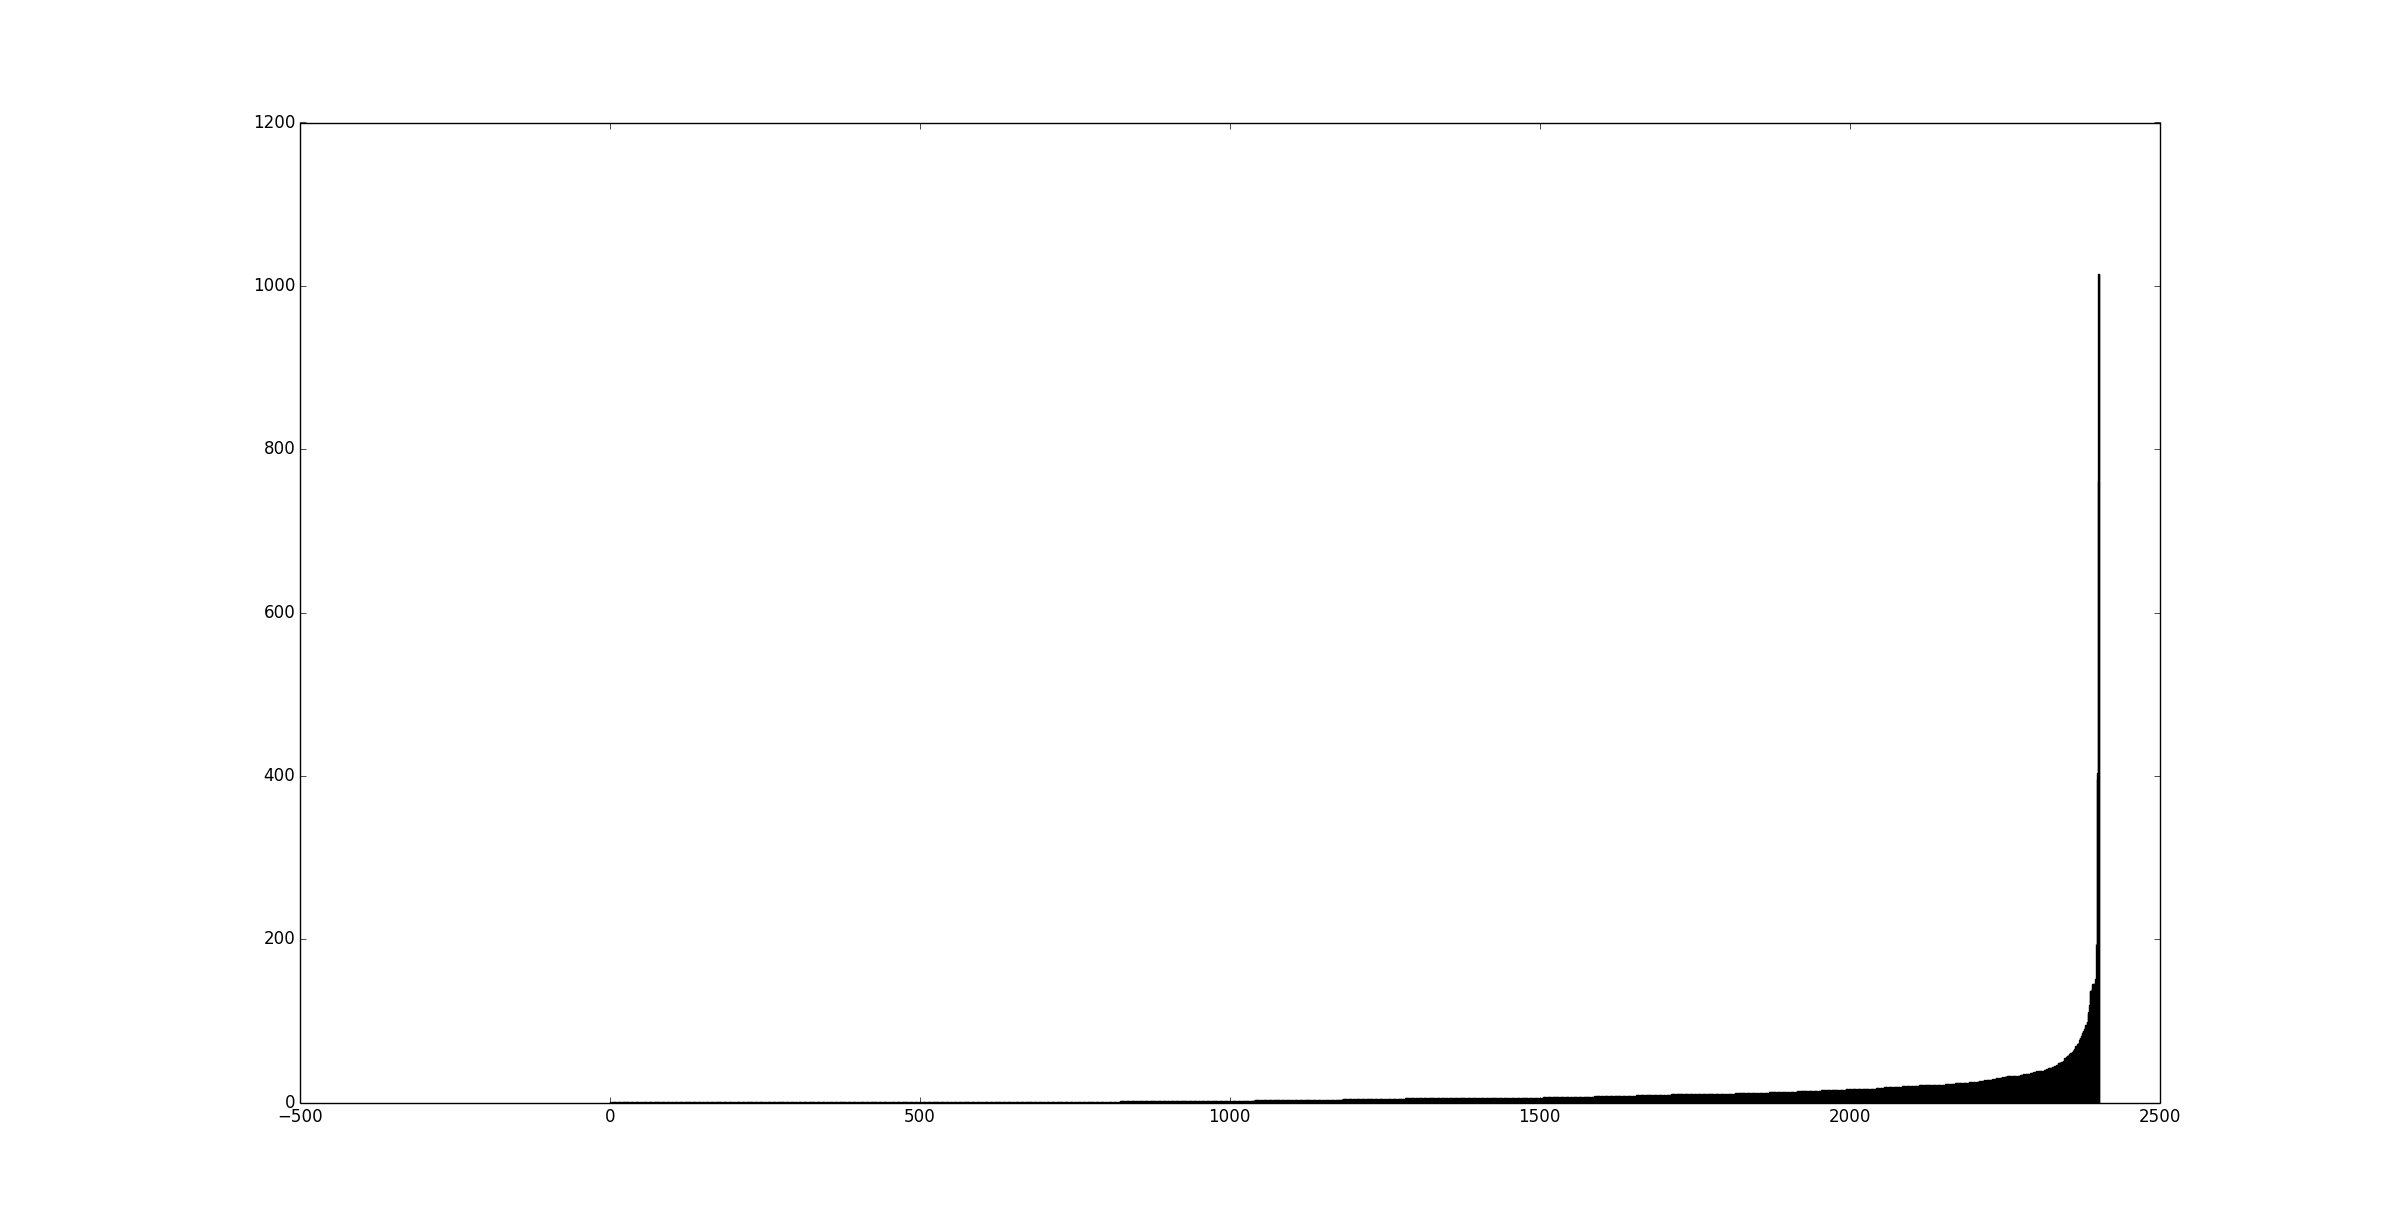
\includegraphics[width=0.5\textwidth, height=5cm]{positions}
\caption{Positions of tweet in text.}
\label{fig:positions}
\end{figure}
\improvement{Add labels to axes in graph}


\subsubsection{Percentage match}

Next, we did a percentage match with the text of the article. This was a bag-of-words check using unigrams from the tweet and the document. The order of the words in the tweet or the text did not matter. The results we got seem to suggest that a lot of significant words in the tweet are in fact present in the article. The minimum percentage match obtained was 60\%. However, since the order of the words did not matter, this result can  be traced back to the fact that tweet is based on the same topic as the document. \improvement{Calculate the number of words in common in this case}

\subsubsection{Percentage matching inside a window in the article text}

The next analysis was to check for a significant word matching inside a two or three sentence window inside the article text. We used a three sentence long window using the sentence boundary information obtained during preprocessing. After the text of the window was extracted, we performed a similar analysis as the last one, except on a smaller set of sentences. Again, the order of the unigrams didn't matter. Next, the matching percentages from all such windows in the articles were compared and the maximum out of these was considered for the highest match percentage and match position for the final results. The result from this experiment is shown in \figref{fig:percentages}. 

\begin{figure}[htbp]
\centering
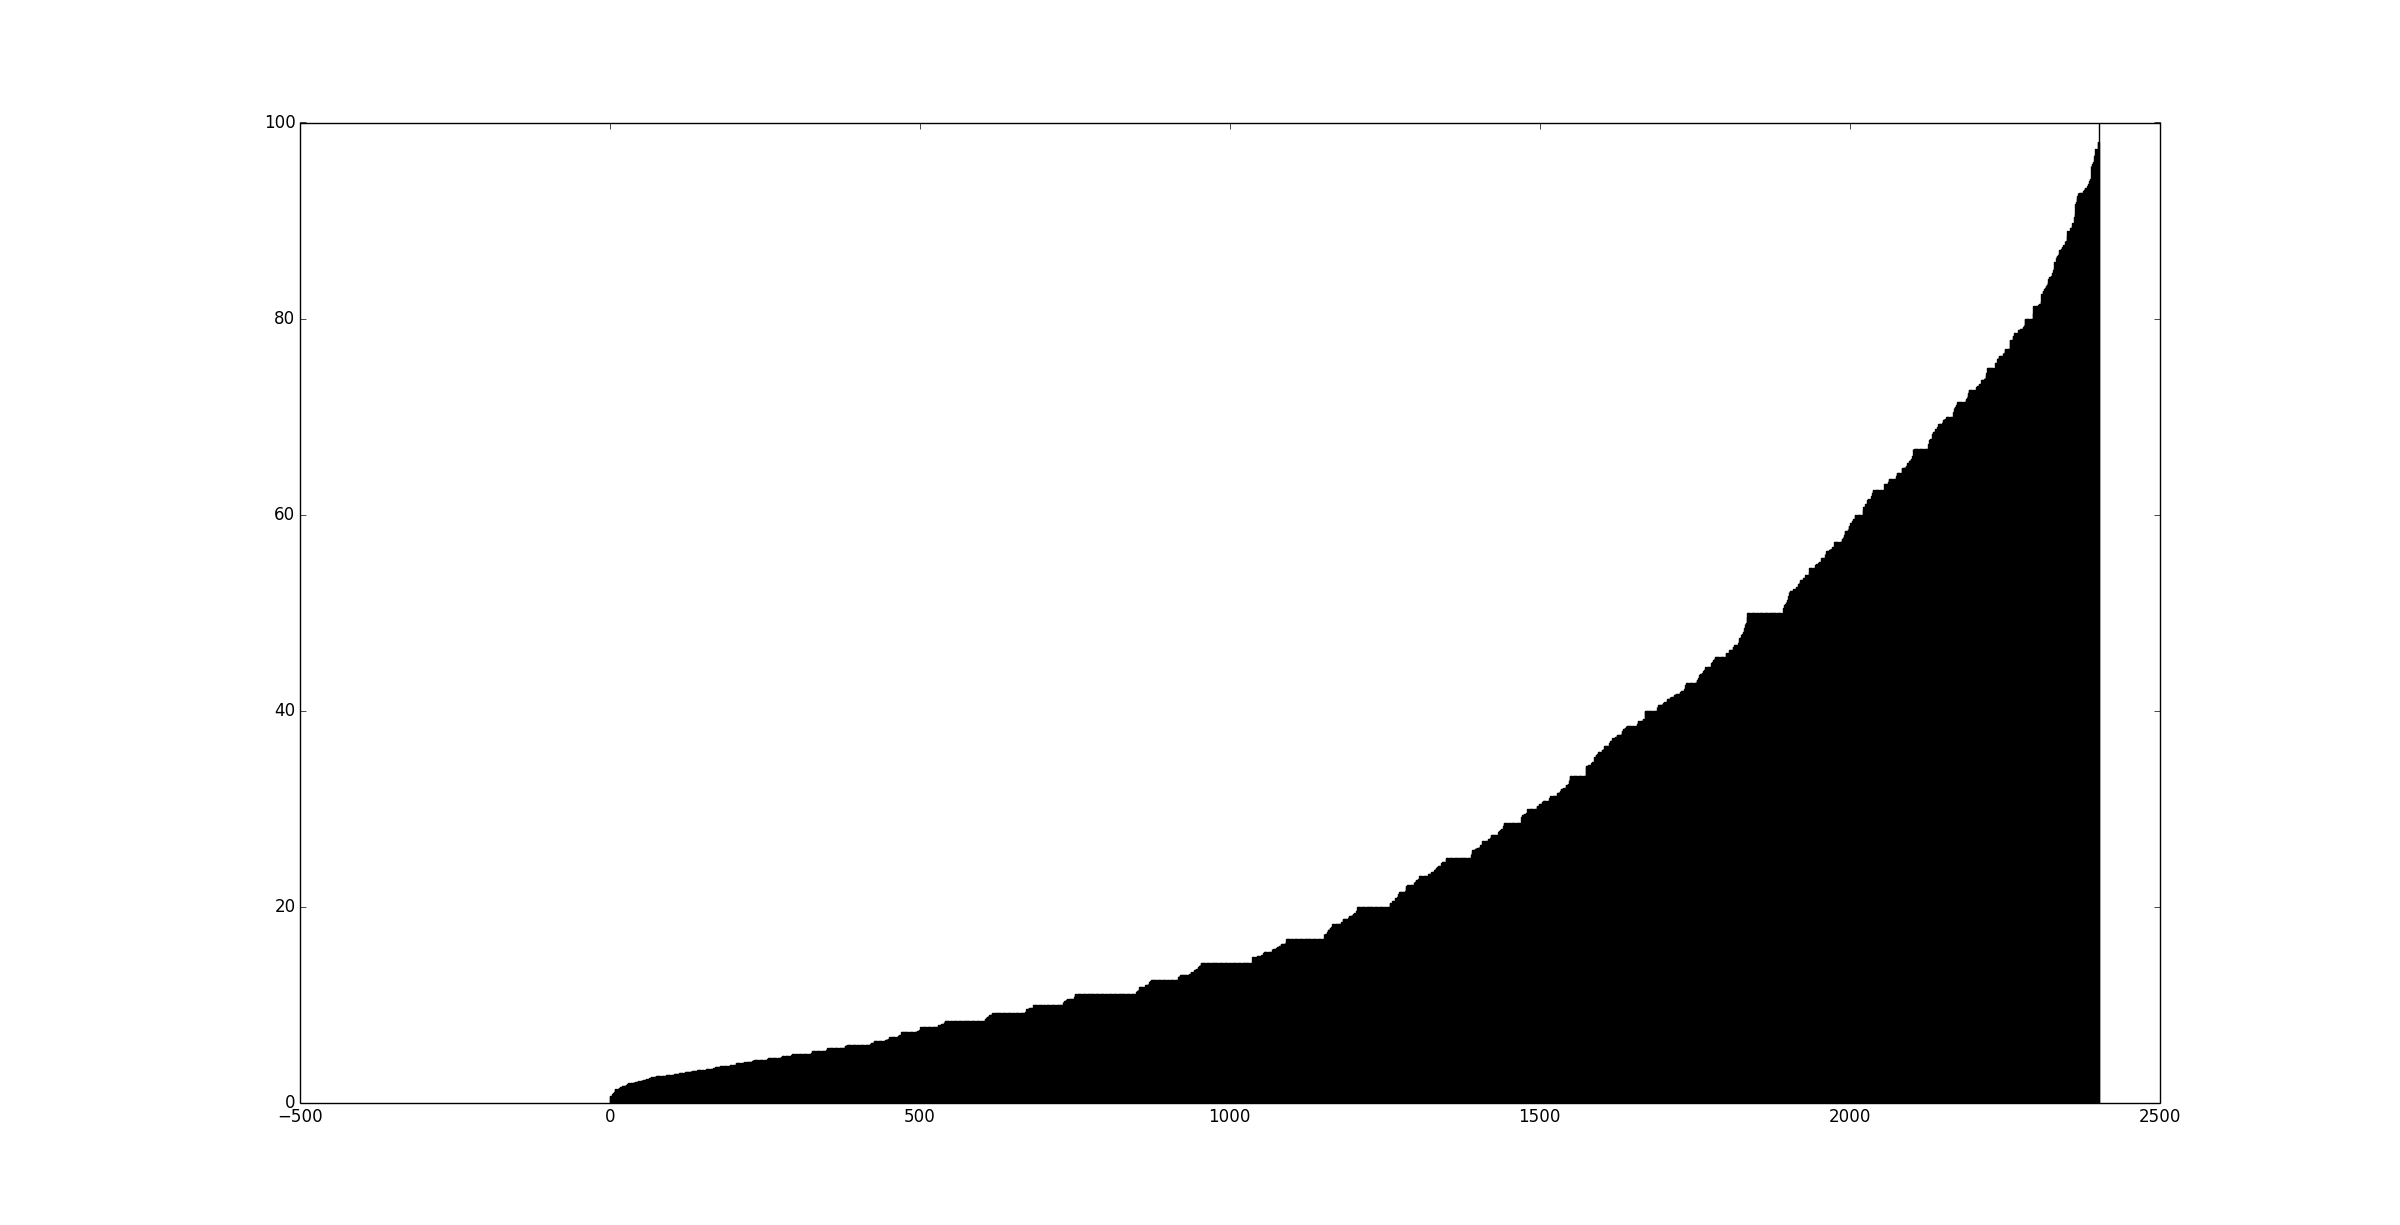
\includegraphics[width=0.5\textwidth, height=5cm]{percentages}
\caption{Percentages of common words in tweet and text.}
\label{fig:percentages}
\end{figure}
\improvement{Add labels to axes in graph}

\subsubsection{Least Common Subsequence match inside a window for the text}

The percentage match analyses were a bag-of-words approach disregarding the order of the words inside the texts and tweets. To respect the order of the words in the sentence of the tweet, we also used the least common subsequence algorithm between the tweet text and the document text. This subsequence matching was done inside a sentence window of 5 sentences. Again, the final result for the article was the window in which the maximum percentage was recorded among all windows. The percentage match was calculated against the number of words in the tweet, as found in the least common subsequence calculated between the two texts. These numbers are shown in \figref{lcs_doc}.

\begin{figure}[htbp]
\centering
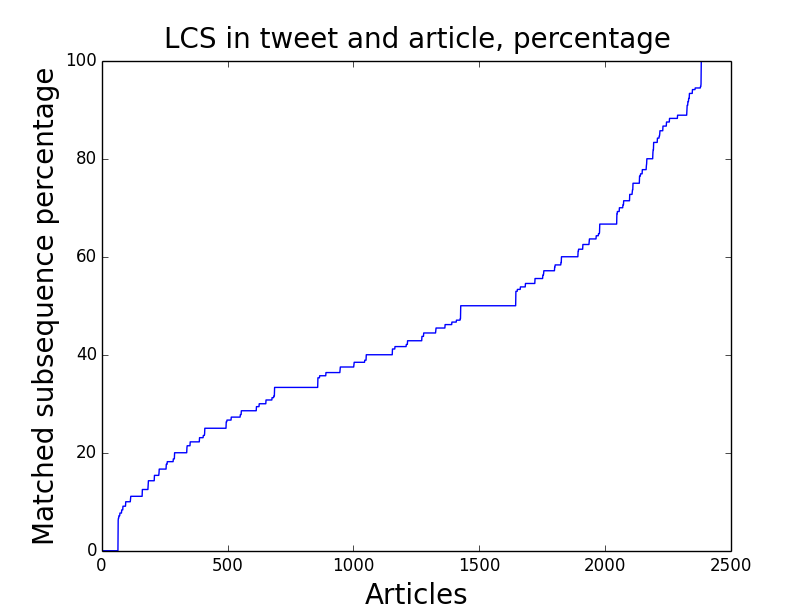
\includegraphics[width=0.5\textwidth, height=5cm]{lcs_doc}
\caption{Percentages of words matching in tweet and document text using an LCS algorithm.}
\label{fig:lcs}
\end{figure}
\improvement{Add labels to axes in graph}



\subsection{Subjectivity and Formality}
\change{should subjectivity be included?}

To achieve this, the degree of formality of the text was calculated with the help of some other studies. The formality lexicon gives was generated by \newcite{brooke2013multi} and can be used to measure formality of a given text. The lexicon consists of words and phrases and the degree of formality for their occurrence. Thus, more formal words marked on a positive scale and informal words like those occurring in colloquial language are marked on a negative scale. Using the formality and subjectivity lexicons, the degree of subjectivity and formality of each individual article was calculated. 

The degree of subjectivity returned a count per of the number of words present in the article that suggested an opinion per article. This number was normalized with the length of the article, and the degree of subjectivity was calculated per 10 words of an article. For this result, only the strong subjective entries in the lexicon were used to better differentiate between subjective and non-subjective articles.

\begin{equation}
\resizebox{.9\hsize}{!}{$formalityScore = \frac{| unigramsArticle \cap formalitySet |}{| unigramsArticle |} * 10$}
\end{equation}

The formality lexicon gave positive weights for formal expressions and negative for informal expressions. After calculating the formality weights for all articles, it was observed that they all had a total negative normalized weight, meaning a lot more informal expressions were getting matched. Hence, we used just the formal word occurrences for calculating the weight. Thus, above a certain cut-off weight, the article could be considered formal, else would be considered informal.

All the weights from both lexicons were averaged out over the articles relating to a single search term(or hashtag), and then ranked accordingly. The ranking showed that for subjectivity ranking over hashtags, films and music related hashtags are at the top, which would be the natural intuition given the nature of the topics. On the other hand, in the formality ranking, the hashtags relating to political issues had the highest formality ranking, while the hashtags for film titles, pop culture are all at the bottom. This also correlates with intuition about the topics. As a sanity check, we also looked at articles at the extreme points of the both the graphs. The texts of these articles suggested that they were consistent with the numbers.

Correlation between the rankings of hashtags given by both these experiments was calculated, and the Kendall’s tau for this was 0.09 with a p-value of 0.34. The low correlation suggests that these two ways of evaluating subjectivity and formality are independent. The p-value suggests that there is not enough evidence to prove a correlation between subjectivity and formality of an article.

% \section{Evaluation}
% \todo{Perform and Write}

\section{Results}
\todo{Discuss
* Implication of results - tweet can't be extracted

* Correlation of formality and lcs scores
}


\section{Conclusion}
\todo{Write}

\section{Future Work}
\todo{write

* Classifying tweets based on intent, and being able to generate tweet might be generated from a template}

\section*{Acknowledgments}

% include your own bib file like this:
\bibliographystyle{acl}
\bibliography{acl2015}

\end{document}